\subsubsection{Đường ống dữ liệu văn bản pháp luật}

Khi làm việc với bài toán dữ liệu thực tế,
việc thu thập dữ liệu có thách thức phụ thuộc vào nguồn dữ liệu.
Vào ngày 24/05/2026,
nguồn dữ liệu văn bản pháp luật được thay đổi cả hệ thống,
API và giao diện.
Do sự thay đổi lớn
về dữ liệu thu thập nên hệ thống cần xử lý lại toàn bộ các bước trong luồng dữ liệu.

% Giao diện nguồn dữ liệu văn bản pháp luật mới:

\begin{figure}[H]
\centering
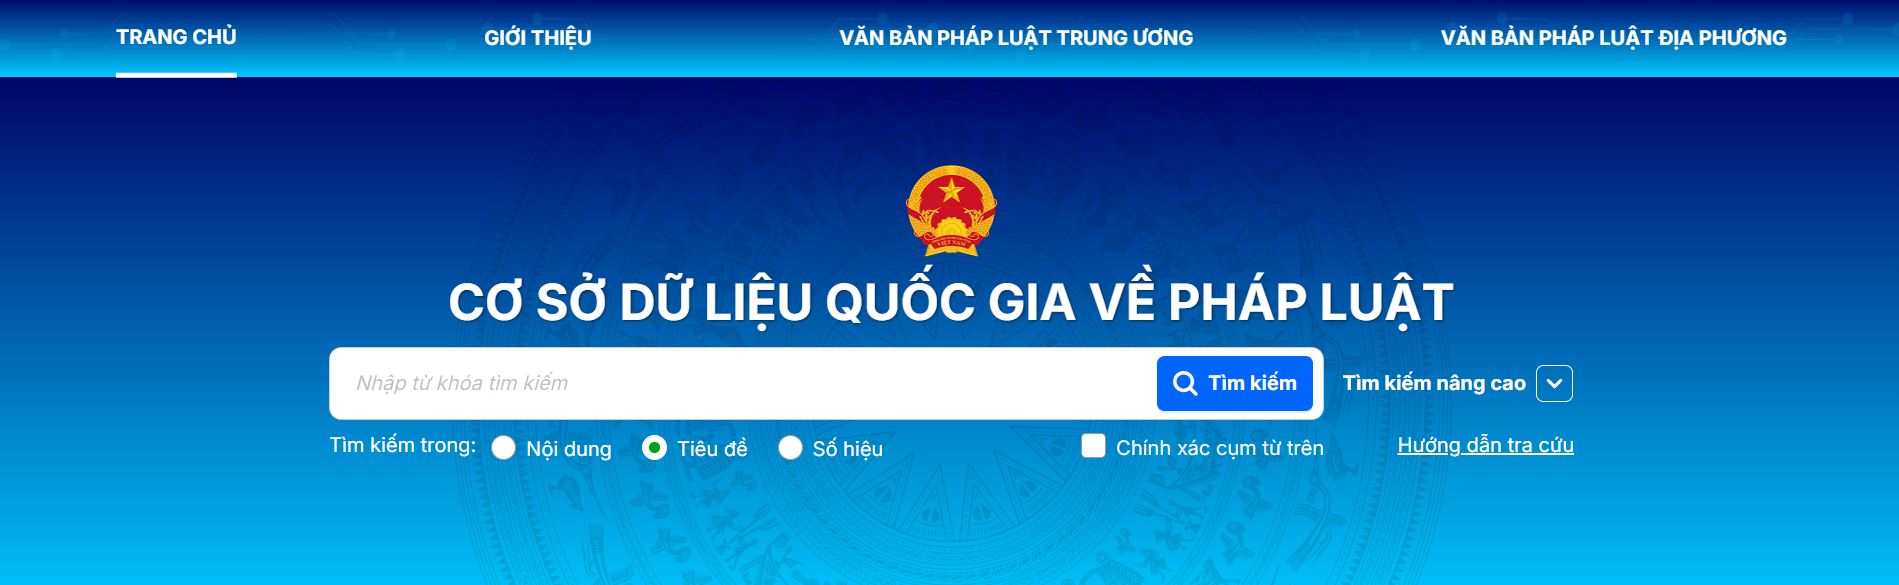
\includegraphics[width=0.7\textwidth]{pictures/vbpl-search.png}
\caption[Giao diện trang tìm kiếm của nguồn dữ liệu văn bản pháp luật mới]{Giao diện trang tìm kiếm của nguồn dữ liệu văn bản pháp luật mới (Nguồn: \cite{vbpl})}
\end{figure}

% Sơ đồ tổng quan luồng dữ liệu văn bản pháp luật mới:

\begin{figure}[H]
\centering
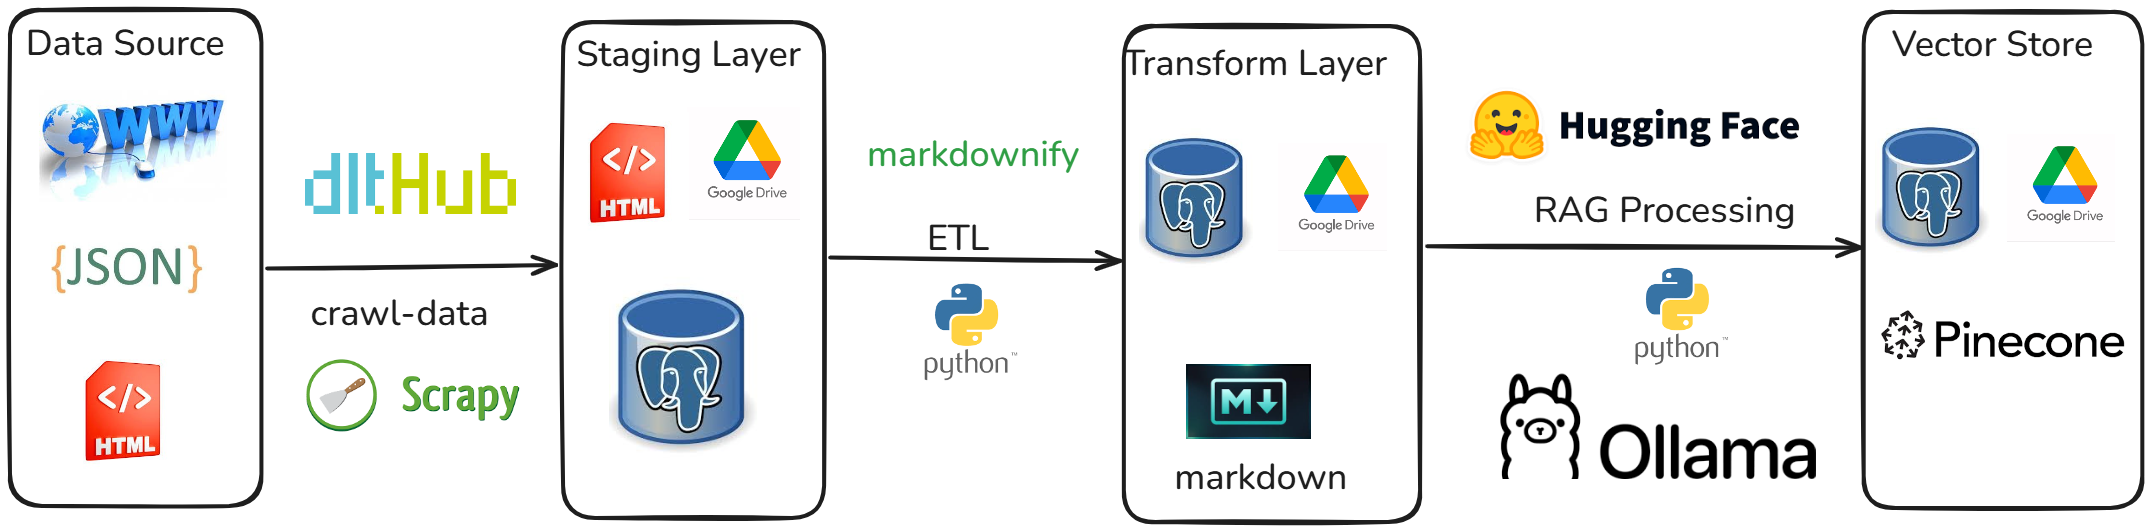
\includegraphics[width=0.7\textwidth]{pictures/Data-Pipeline-VBPL.excalidraw.png}
\caption{Sơ đồ tổng quan luồng dữ liệu văn bản pháp luật mới}
\end{figure}

Các bước thực hiện cũ:

\begin{figure}[H]
\centering
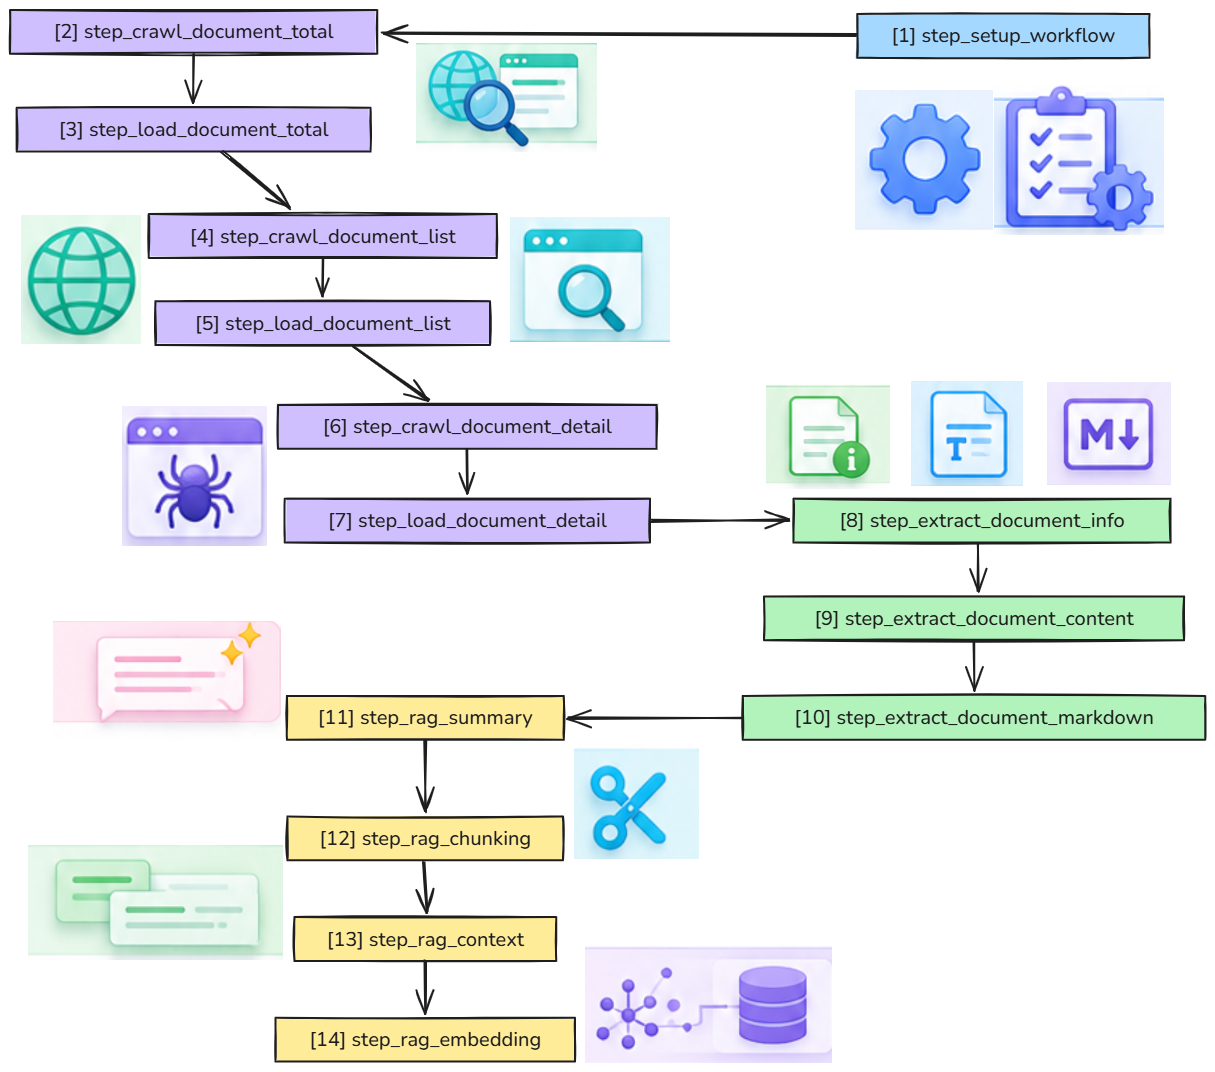
\includegraphics[width=0.95\textwidth]{pictures/step0.excalidraw.png}
\caption{Sơ đồ các bước thực hiện của quy trình cũ}
\end{figure}

% Mô tả các bước thực hiện cũ:

Quá trình luồng dữ liệu được chia thành 3 giai đoạn: Thu thập dữ liệu, tiền xử lý văn bản và tích hợp quy trình RAG.

% \textbf{Giai đoạn Khởi tạo:}
\begin{itemize}
\item \texttt{step\_setup\_workflow} cập nhật danh sách và thứ tự các bước (workflow) vào CSDL.
\end{itemize}

% \textbf{Giai đoạn Thu thập Dữ liệu:}
\begin{itemize}
\item \texttt{step\_crawl\_document\_total} và \texttt{step\_load\_document\_total}: thu thập tổng số lượng văn bản pháp luật hiện có trên hệ thống web.
\begin{figure}[H]
\centering
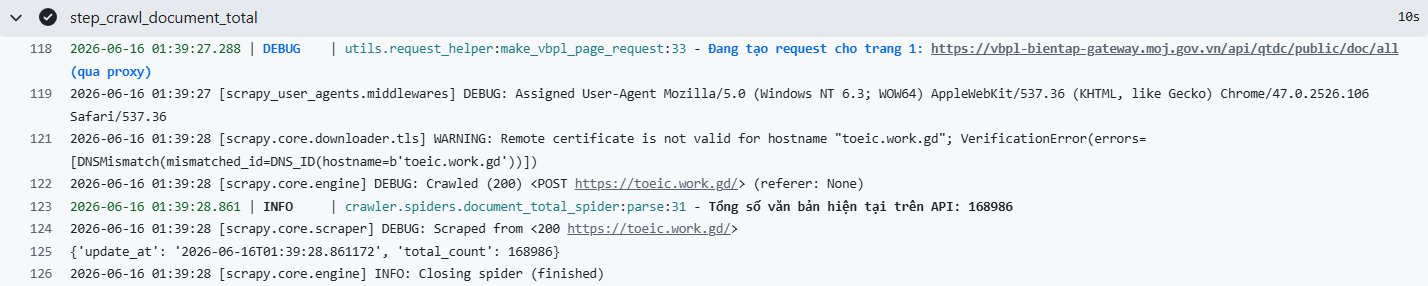
\includegraphics[width=0.95\textwidth]{pictures/data-pipeline-vbplnew-step-crawl-document-total.png}
\caption{Thu thập tổng số lượng văn bản pháp luật}
\end{figure}

\item \texttt{step\_crawl\_document\_list} và \texttt{step\_load\_document\_list}: Dựa vào sự chênh lệch tổng số lượng, tính toán số trang cần quét và thu thập danh sách các \texttt{item\_id}.
\begin{figure}[H]
\centering
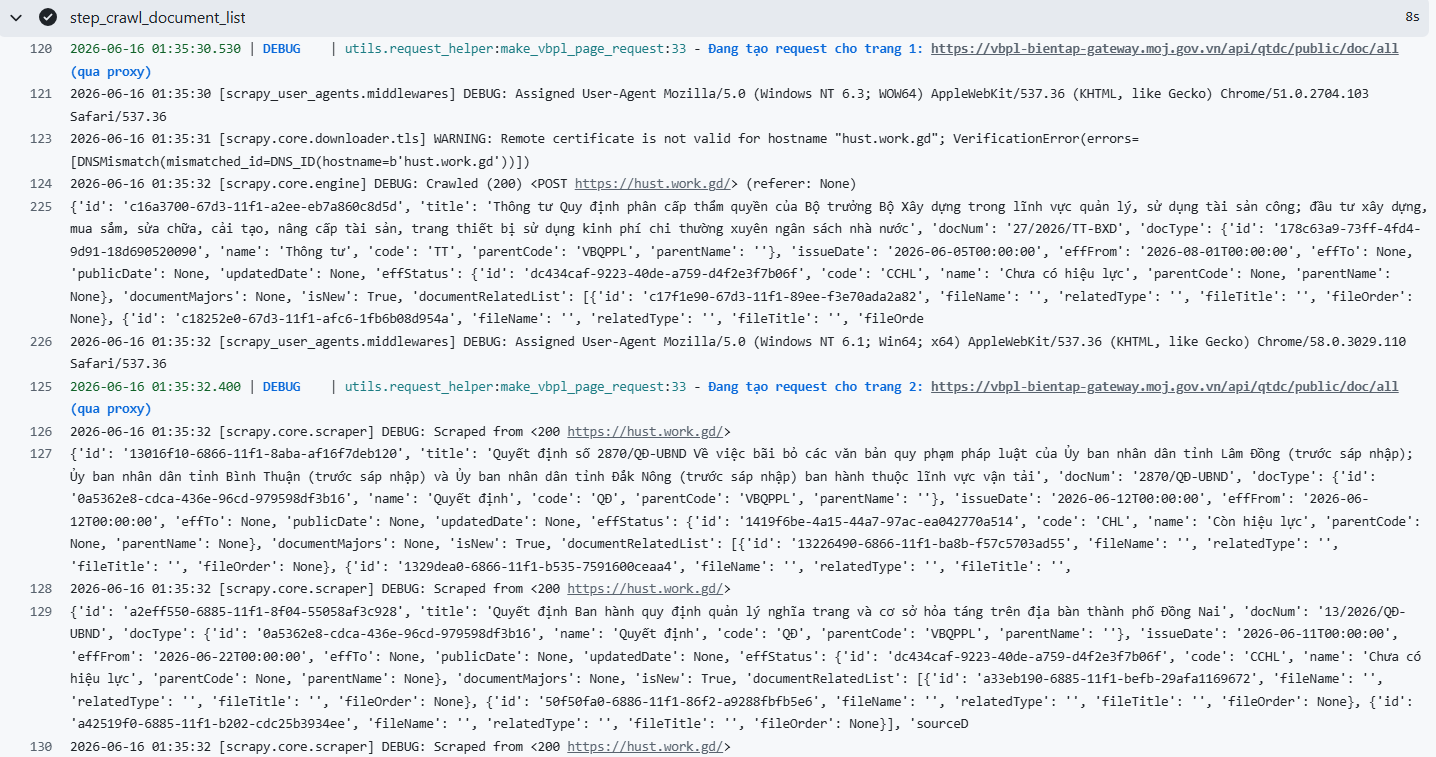
\includegraphics[width=0.95\textwidth]{pictures/data-pipeline-vbplnew-step-crawl-document-list.png}
\caption{Quét danh sách các văn bản pháp luật}
\end{figure}
\begin{figure}[H]
\centering
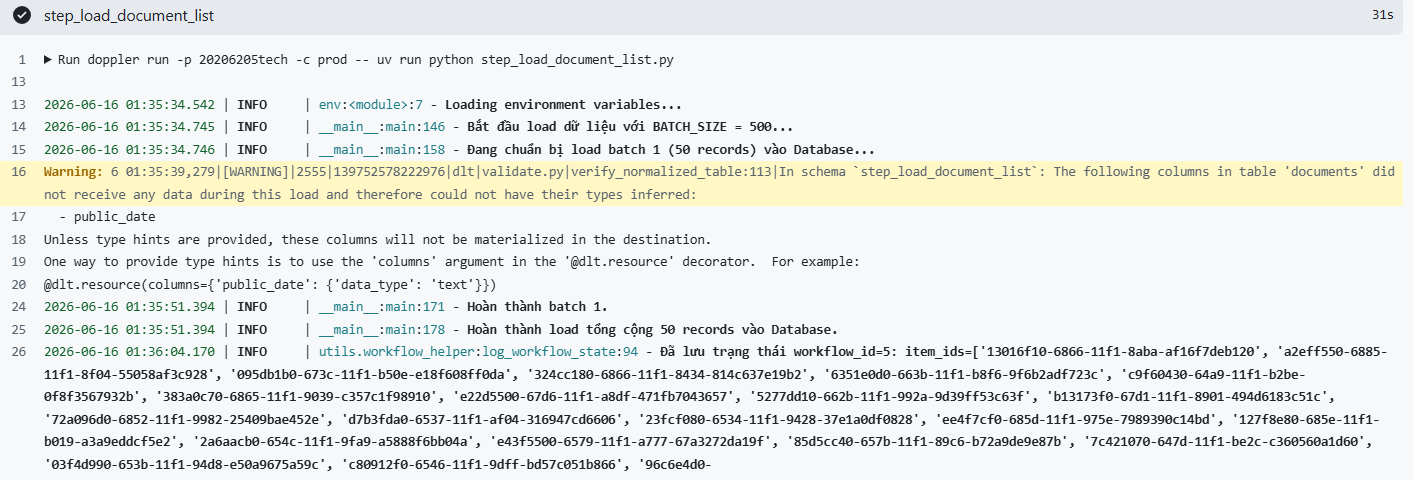
\includegraphics[width=0.95\textwidth]{pictures/data-pipeline-vbplnew-step-load-document-list.png}
\caption{Nạp danh sách văn bản vào CSDL}
\end{figure}

\item \texttt{step\_crawl\_document\_detail} và \texttt{step\_load\_document\_detail}: tải mã nguồn trang chi tiết của từng văn bản và Upload các file HTML gốc này lên Google Drive, đồng thời lưu \texttt{drive\_id} và mã băm MD5 hash vào database để quản lý thay đổi.

\begin{figure}[H]
\centering
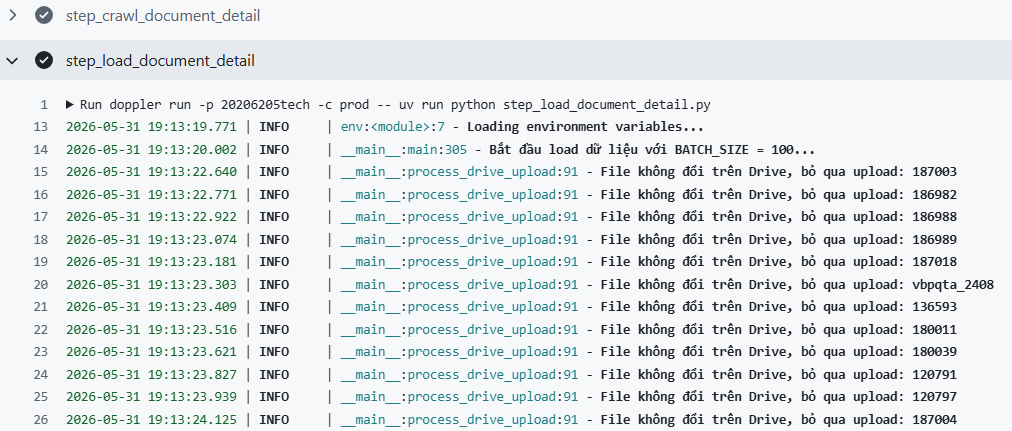
\includegraphics[width=0.9\textwidth]{pictures/data-pipeline-vbplnew-step-crawl-document-detail-step-load-document-detail.png}
\caption{Tải và lưu trữ mã nguồn HTML trang chi tiết văn bản}
\end{figure}
\end{itemize}

% \textbf{Giai đoạn Tiền xử lý Dữ liệu:}
\begin{itemize}
\item \texttt{step\_extract\_document\_info}: từ file HTML, bóc tách các siêu dữ liệu quan trọng (Metadata) như: số hiệu, cơ quan ban hành, ngày có hiệu lực, người ký, \dots và lưu vào database.
\item \texttt{step\_extract\_document\_content}: Làm sạch file HTML, cắt bỏ các phần thừa (header, footer, menu) và chỉ giữ lại phần nội dung (thẻ \texttt{div\#toanvancontent}).
\item \texttt{step\_extract\_document\_markdown}: Chuyển đổi file HTML đã làm sạch sang định dạng Markdown.
\begin{figure}[H]
\centering
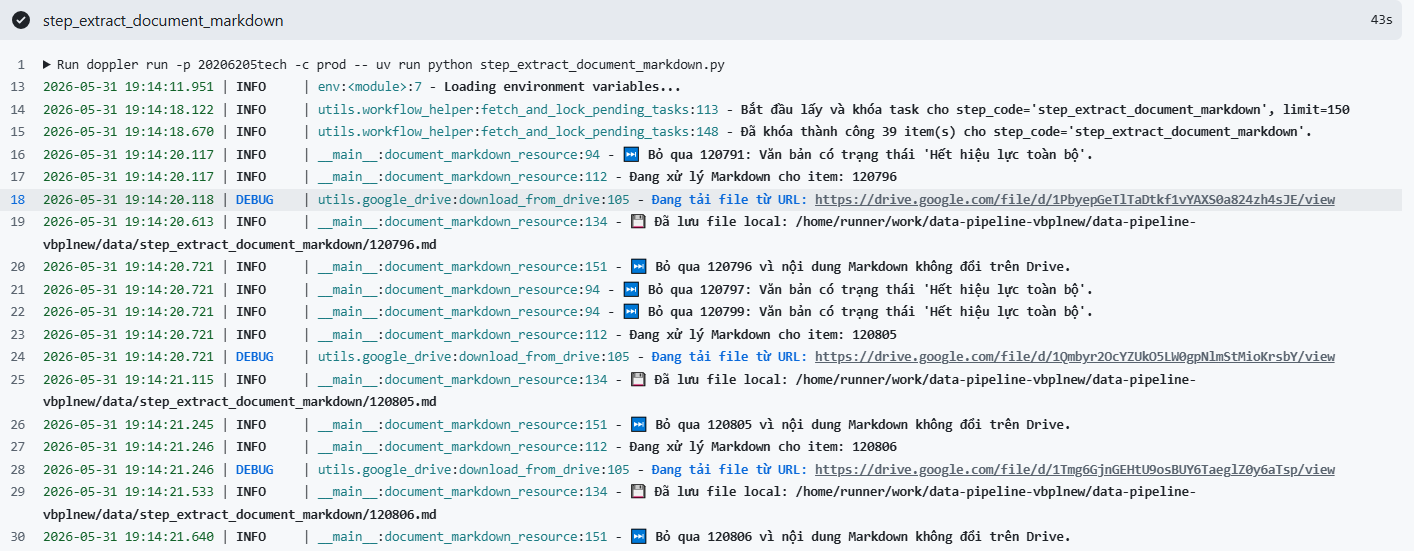
\includegraphics[width=0.95\textwidth]{pictures/data-pipeline-vbplnew-step-extract-document-markdown.png}
\caption{Chuyển đổi nội dung HTML đã làm sạch sang Markdown}
\end{figure}
\end{itemize}

% \textbf{Giai đoạn Tích hợp RAG pipeline:}
\begin{itemize}
\item \texttt{step\_rag\_summary}: Sử dụng LLM viết một bản tóm tắt ngắn gọn mô tả bức tranh toàn cảnh của văn bản pháp luật đó.
\begin{figure}[H]
\centering
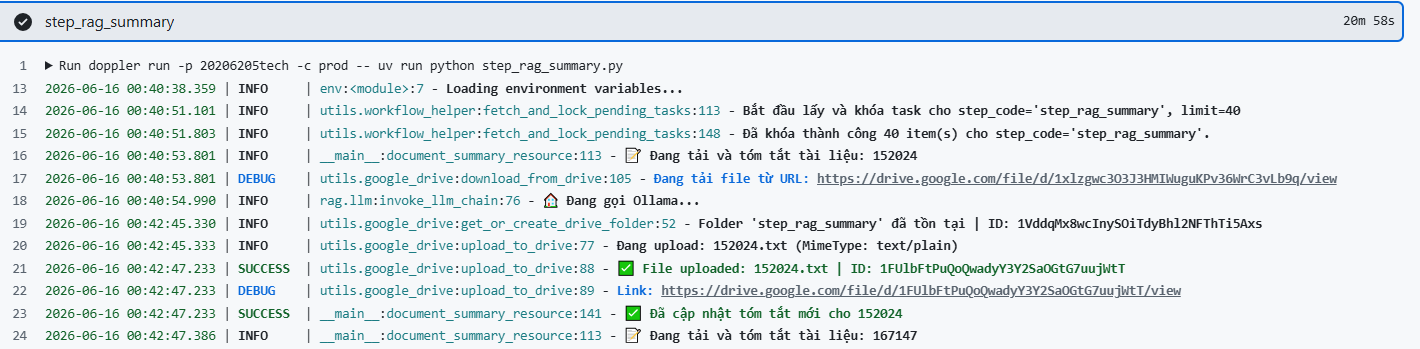
\includegraphics[width=0.95\textwidth]{pictures/data-pipeline-vbplnew-step-rag-summary.png}
\caption{Tự động tóm tắt văn bản bằng mô hình LLM}
\end{figure}

\item \texttt{step\_rag\_chunking}: Chạy Semantic Chunking. LLM sẽ dựa vào bản tóm tắt và nội dung chi tiết để quyết định các \enquote{điểm cắt} tối ưu, chia nhỏ văn bản thành các đoạn (chunks) sao cho không bị đứt gãy ý nghĩa.
\begin{figure}[H]
\centering
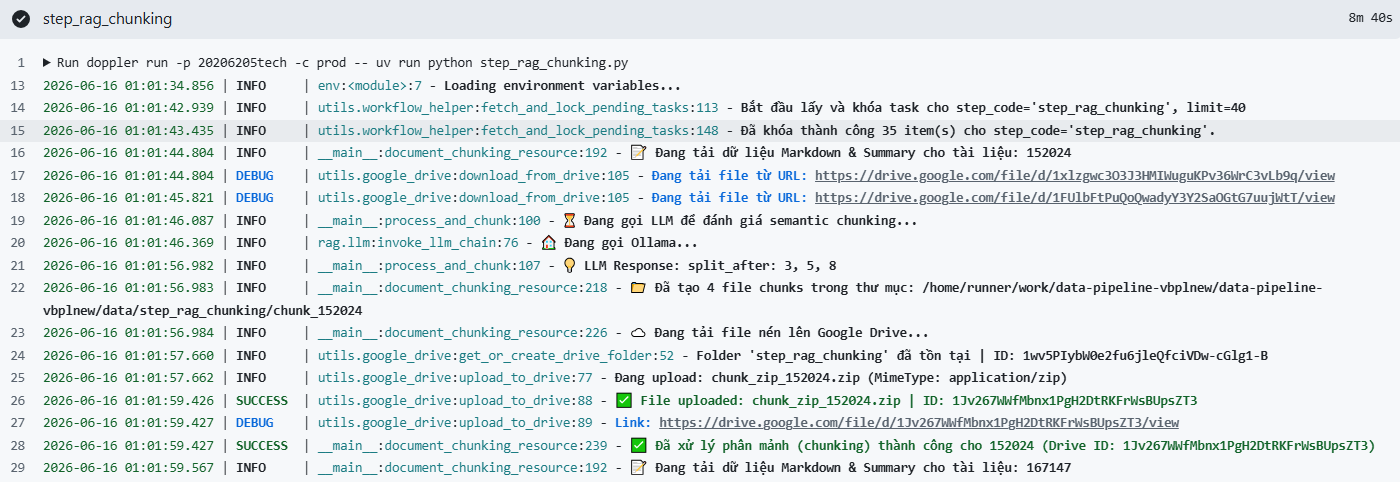
\includegraphics[width=0.99\textwidth]{pictures/data-pipeline-vbplnew-step-rag-chunking.png}
\caption{Chia nhỏ văn bản dựa trên ý nghĩa (Semantic Chunking)}
\end{figure}

\item \texttt{step\_rag\_context}: Đây là bước chống mất ngữ cảnh. LLM sẽ sinh ra ngữ cảnh cho từng đoạn chunk nhỏ vừa được cắt, đảm bảo mỗi chunk đều có thể đứng độc lập khi được tìm kiếm.
\begin{figure}[H]
\centering
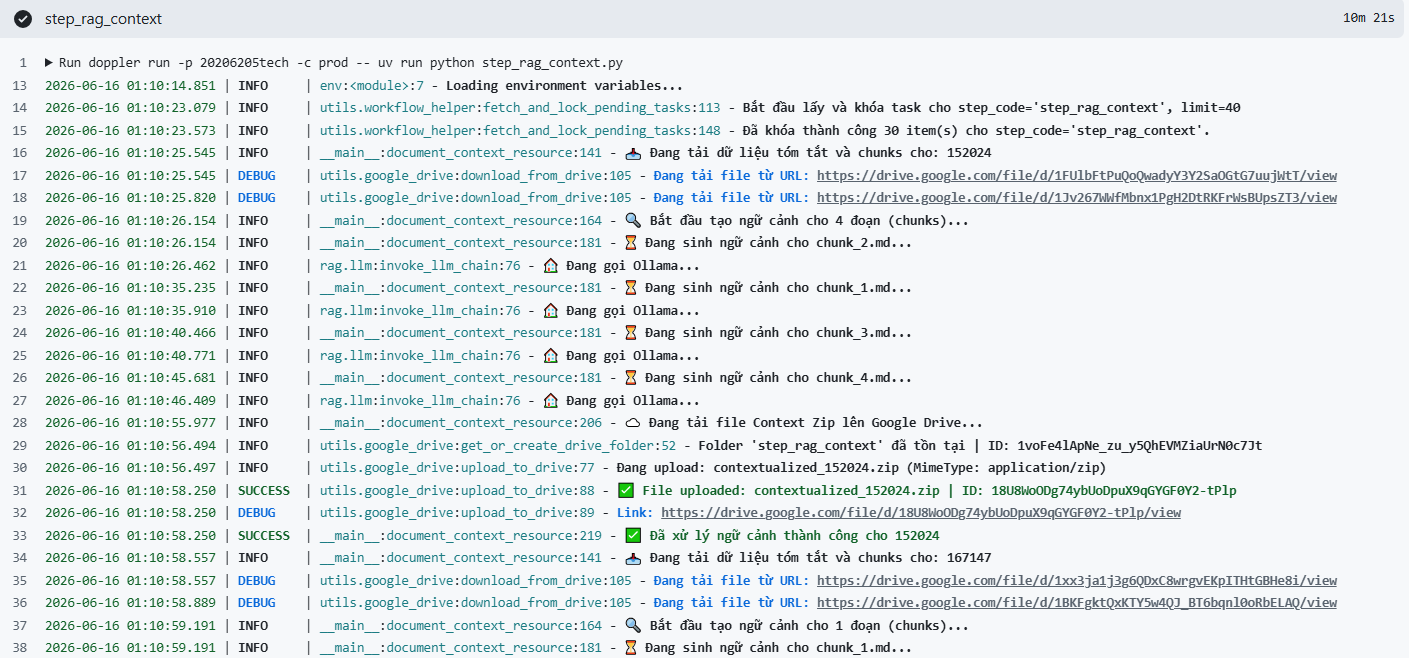
\includegraphics[width=0.99\textwidth]{pictures/data-pipeline-vbplnew-step-rag-context.png}
\caption{Làm giàu ngữ cảnh cho từng đoạn văn bản nhỏ}
\end{figure}

\item \texttt{step\_rag\_embedding}: Sử dụng mô hình HuggingFace (\texttt{keepitreal/vietnamese-sbert})
để biến đổi các đoạn văn bản (đã có ngữ cảnh) thành vector đa chiều và lưu trữ vào VectorDB (Pinecone).
\begin{figure}[H]
\centering
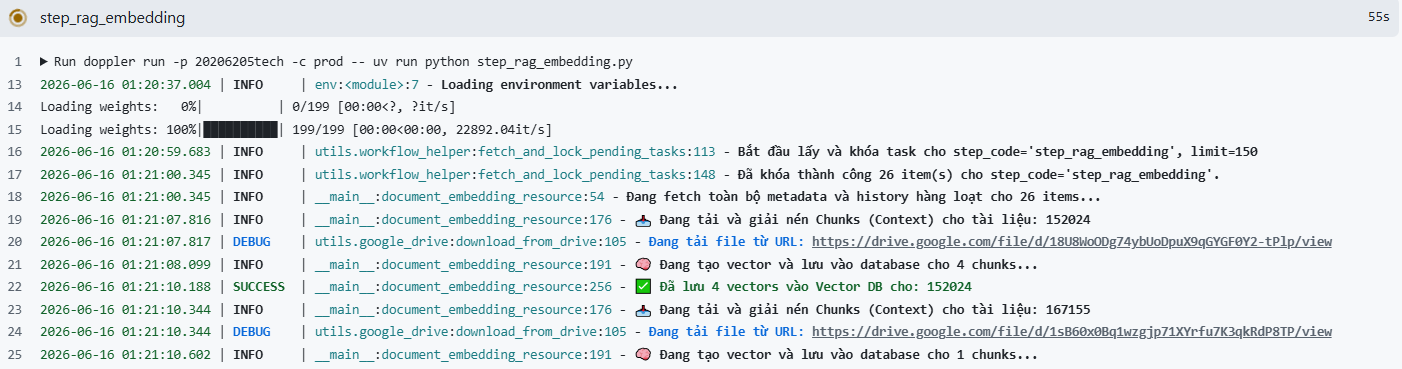
\includegraphics[width=0.99\textwidth]{pictures/data-pipeline-vbplnew-step-rag-embedding.png}
\caption{Nhúng văn bản (Embedding) và lưu vào CSDL Pinecone}
\end{figure}
\end{itemize}

Các bước thực hiện mới:

\begin{itemize}
\item Nhờ vào việc nguồn dữ liệu thay đổi sang hệ thống API mới trả về cấu trúc JSON giàu thông tin, hệ thống không còn cần các bước bóc tách thủ công từ mã nguồn HTML phức tạp, giúp tăng tốc độ xử lý và độ chính xác của dữ liệu.
\item Hệ thống loại bỏ bước \texttt{step\_extract\_document\_info} vì nội dung Metadata chi tiết đã có trong API.
\item Hệ thống loại bỏ bước \texttt{step\_extract\_document\_content} vì nội dung văn bản đã được API trả trong thông tin \texttt{documentContent}.
\end{itemize}

\begin{figure}[H]
\centering
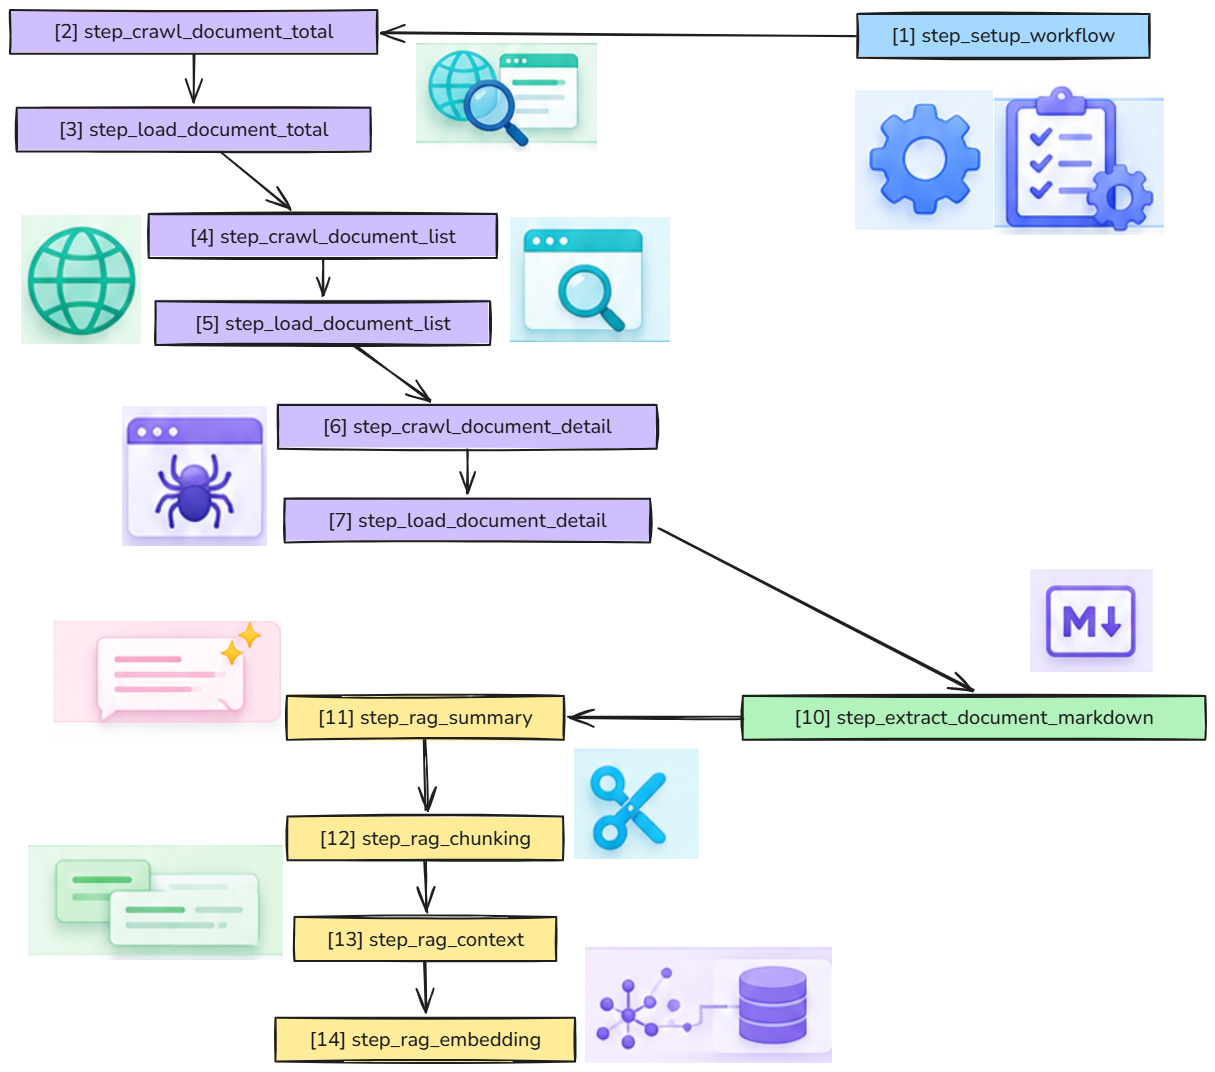
\includegraphics[width=0.6\textwidth]{pictures/step1.excalidraw.png}
\caption{Sơ đồ các bước thực hiện của quy trình mới}
\end{figure}

% \begin{figure}[H]
% \centering
% 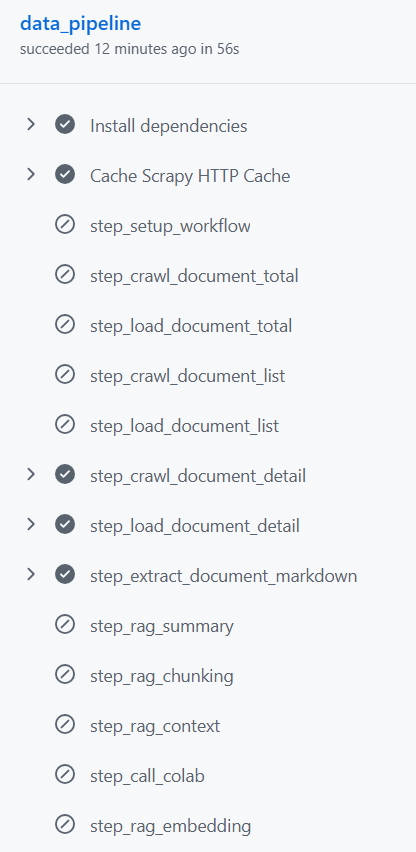
\includegraphics[width=0.6\textwidth]{pictures/github-action-vbpl-v2.png}
% \caption{Sơ đồ cấu hình GitHub Actions vận hành workflow mới}
% \end{figure}

Kết quả vận hành thành công đường ống dữ liệu văn bản pháp luật mới:

\begin{figure}[H]
\centering
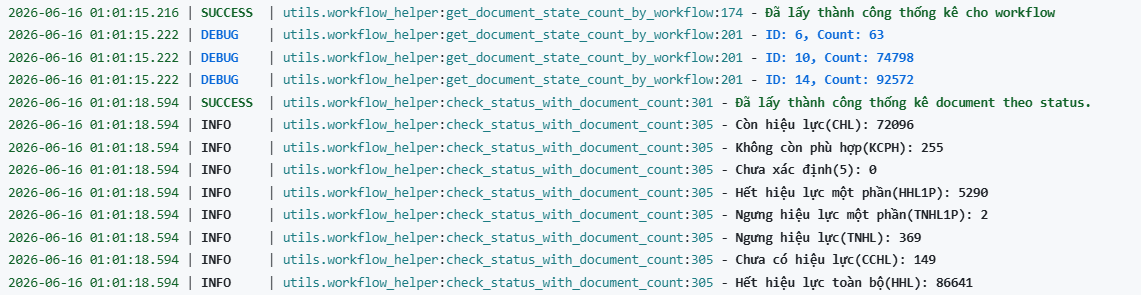
\includegraphics[width=0.95\textwidth]{pictures/data-pipeline-vbplnew-done-1.png}
\caption{Kết quả chạy các bước luồng dữ liệu VBPL mới (Phần 1)}
\end{figure}

Từ kết quả chạy các bước luồng dữ liệu VBPL mới,
trong database postgres hiện đang có
kết quả
số lượng tài liệu chi tiết theo từng trạng thái hiệu lực:

\begin{itemize}
\item Còn hiệu lực (CHL): 72.096
\item Không còn phù hợp (KCPH): 255
\item Chưa xác định (5): 0
\item Hết hiệu lực một phần (HHL1P): 5.290
\item Ngưng hiệu lực một phần (TNHL1P): 2
\item Ngưng hiệu lực (TNHL): 369
\item Chưa có hiệu lực (CCHL): 149
\item Hết hiệu lực toàn bộ (HHL): 86.641
\end{itemize}

\begin{figure}[H]
\centering
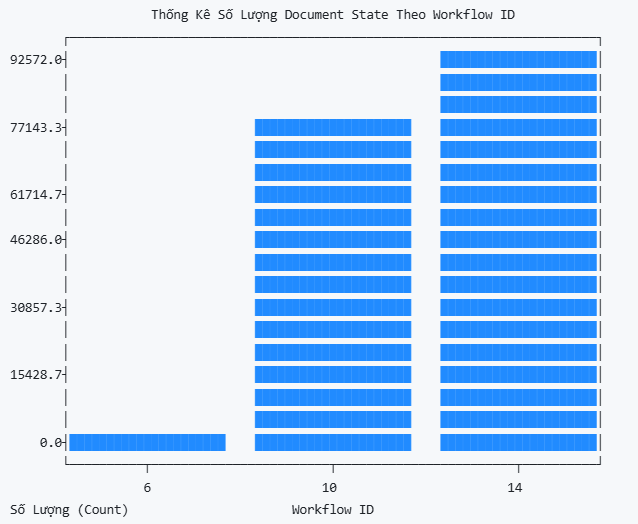
\includegraphics[width=0.9\textwidth]{pictures/data-pipeline-vbplnew-done-2.png}
\caption{Kết quả chạy các bước luồng dữ liệu VBPL mới (Phần 2)}
\end{figure}

\begin{figure}[H]
\centering
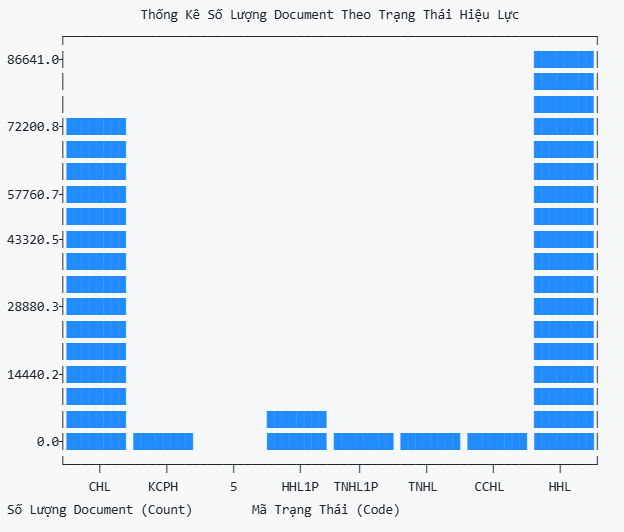
\includegraphics[width=0.9\textwidth]{pictures/data-pipeline-vbplnew-done-3.png}
\caption{Kết quả chạy các bước luồng dữ liệu VBPL mới (Phần 3)}
\end{figure}
